\input ../preamble

\begin{document}

{\Huge

  \centerline{\bf TTIC 31230, Fundamentals of Deep Learning}
  \bigskip
  \centerline{David McAllester, Winter 2018}
  \vfill
  \centerline{Controlling Gradients}
  \vfill
  \vfill
  \centerline{Vanishing and Exploding Gradients}
  \vfill
  \centerline{Initialization}
  \vfill
  \centerline{Batch Normalization}
  \vfill
  \centerline{Residual Networks}
  \vfill
  \centerline{Gated RNNs}

\slide{Vanishing and Exploding Gradients}
~
\vfill
\centerline{Causes of Vanishing and Exploding Gradients:}
\vfill
\centerline{Activation function saturation}
\vfill
\centerline{Repeated multiplication by network weights}
\vfill

\slide{Activation Function Saturation}

Consider the sigmoid activation function $1/(1+ e^{-x})$.

\vfill
\centerline{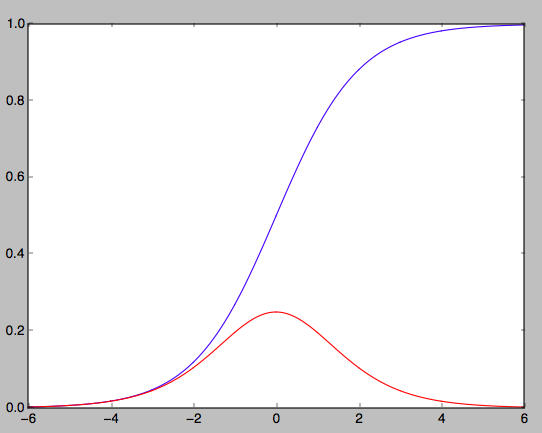
\includegraphics[width= 4.0in]{../images/sigmoid2}}


\vfill
The gradient of this function is quite small for $|x| > 4$.

\vfill
In deep networks backpropagation can go through many sigmoids and
the gradient can ``vanish''

\slide{Activation Function Saturation}

$\mathrm{Relu}(x) = \max(x,0)$

\vfill
\centerline{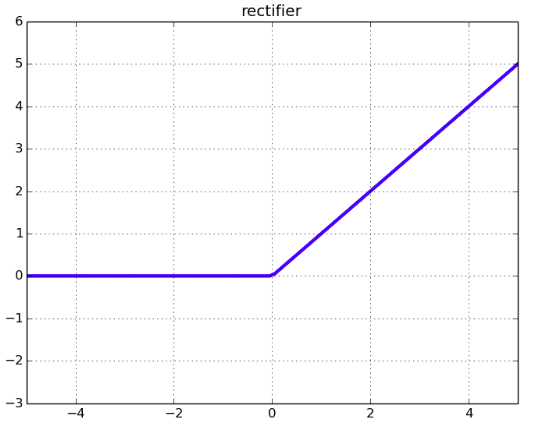
\includegraphics[width= 4.0in]{../images/relu}}

\vfill
The Relu does not saturate at positive inputs (good) but is completely saturated at negative inputs (bad).

\vfill
Alternate variations of Relu still have small gradients at negative inputs.

\slide{Repeated Multiplication by Network Weights}

Consider a deep CNN.

$$L_{i+1} = \mathrm{Relu}(\mathrm{Conv}(\Phi_i,L_i))$$

\vfill
For $i$ large, $L_i$ has been multiplied by many weights.

\vfill
If the weights are small then the neuron values, and hence the weight gradients, decrease exponentially with depth.

\vfill
If the weights are large, and the activation functions do not saturate, then the neuron values, and hence the weight gradients,
increase exponentially with depth.

\slide{Methods for Maintaining Gradients}

\centerline{Initialization}

\vfill
\centerline{Batch Normalization}

\vfill
\centerline{Highway Architectures (Skip Connections)}

\slide{Methods for Maintaining Gradients}

\centerline{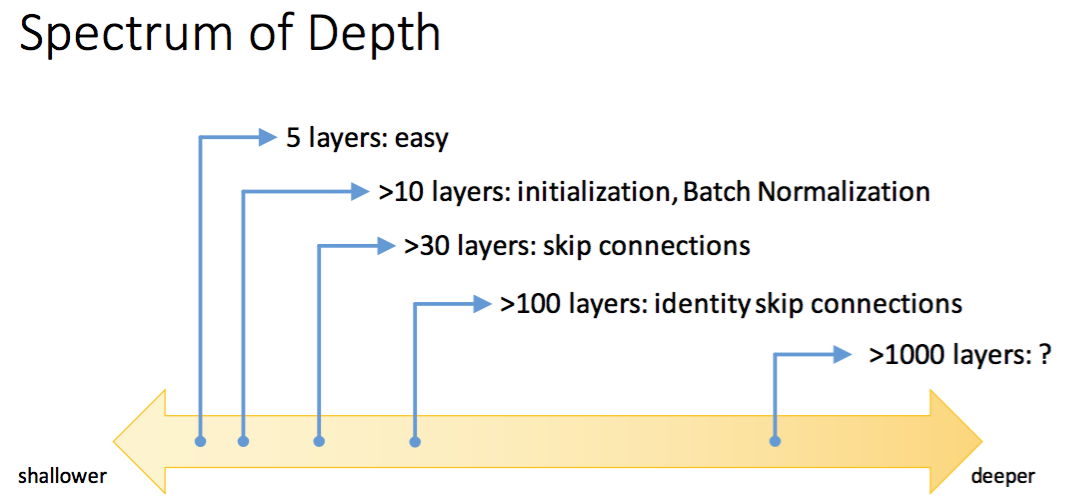
\includegraphics[width = 9in]{../images/DepthSpectrum}}

\centerline{\large Kaiming He}

\slide{}
\centerline{\bf Initialization}
\vfill

\slide{Xavier Initialization}

Initialize a weight matrix (or tensor) to preserve zero-mean unit variance distributions.

\vfill
If we assume $x_i$ has unit mean and zero variance then we want

\vfill
$$y_j = \sum_{j=0}^{N-1} x_i w_{i,j}$$

\vfill
to have zero mean and unit variance.

\vfill
Xavier initialization randomly sets $w_{i,j}$ to be uniform in the interval $\left(-\sqrt{\frac{3}{N}},\;\sqrt{\frac{3}{N}}\right)$.

\vfill
Assuming independence this gives zero mean and unit variance for $y_j$.

\slide{EDF Implementation}

\begin{verbatim}
def xavier(shape):
    sq = np.sqrt(3.0/np.prod(shape[:-1]))
    return np.random.uniform(-sq,sq,shape)
\end{verbatim}

\vfill
This assumes that we sum over all but the last index.

\vfill
For example, an image convolution filter has shape $(W,\;W,\;C_1,C_2)$ and we sum over the first three indices.

\slide{He Initialization}

A Relu nonlinearity reduces the variance.

\vfill
Before a Relu nonlinearity it seems better to use the larger interval $\left(-\sqrt{\frac{6}{N}},\;\sqrt{\frac{6}{N}}\right)$.

\slide{}
\centerline{\bf Batch Normalization}
\vfill

\slide{Normalization}
Given a tensor $x[b,c]$ we define $\tilde{x}[b,c]$ as follows.

\begin{eqnarray*}
  \tilde{x}[b,c]& = & \frac{x[b,c] - \hat{\mu}[c_x]}{\hat{\sigma}[c_x]} \\
  \\
  \\
  \hat{\mu}[c_x] & = & \frac{1}{B} \sum_b\;x[b,c] \\
  \\
  \\
  \hat{\sigma}[c_x] & = & \sqrt{\frac{1}{B-1} \sum_b (x[b,c]-\hat{\mu}[c_x])^2}
\end{eqnarray*}


\vfill
At test time a single fixed estimate of $\mu[c_x]$ and $\sigma[c_x]$ is used.

\slide{Spatial Batch Normalization}

Given a spatial tensor $x[b,i,j,c_x]$ we define $\tilde{x}[b,i,j,c_x]$ as follows.

\begin{eqnarray*}
  \tilde{x}[b,i,j,c_x]& = & \frac{x[b,i,j,c_x] - \hat{\mu}[c_x]}{\hat{\sigma}[c_x]} \\
  \\
  \\
  \hat{\mu}[c_x] & = & \frac{1}{BIJ} \sum_{b,i,j}\;x[b,i,j,c_x] \\
  \\
  \\
  \hat{\sigma}[c_x] & = & \sqrt{\frac{1}{BIJ-1} \sum_{b,i,j} (x[b,i,j,c_x]-\hat{\mu}[c_x])^2}
\end{eqnarray*}

\slideplain{Backpropagation Through Normalization}


\begin{eqnarray*}
  \tilde{x}[b,i,j,c_x]& = & (x[b,i,j,c_x] - \hat{\mu}[c_x])/\hat{\sigma}[c_x] \\
  \\
  x.\mathrm{grad}[b,i,j,c_x] & \pluseq & \tilde{x}.\mathrm{grad}[b,i,j,c_x]/{\hat{\sigma}[c_x]} \\
  \\
  \hat{\mu}.\mathrm{grad}[c_x] & \minuseq & \tilde{x}.\mathrm{grad}[b,i,j,c_x]/{\hat{\sigma}[c_x]} \\
  \\
  \hat{\sigma}.\mathrm{grad}[c_x] & \minuseq & \tilde{x}.\mathrm{grad}[b,i,j,c_x](x[b,i,j,c_x] - \hat{\mu}[c_x])/\hat{\sigma}[c_x]^2
\end{eqnarray*}


\slide{Backpropagation Through Normalization}


\begin{eqnarray*}
  \hat{\mu}[c_x] & = & x[b,i,j,c_x]/(BIJ) \\
  \\
  x.\mathrm{grad}[b,i,j,c_x] & \pluseq & \hat{\mu}.\mathrm{grad}[c_x]/(BIJ) \\
\end{eqnarray*}

\slide{Backpropagation Through Normalization}

\begin{eqnarray*}
  \hat{\sigma}[c_x] & = & \sqrt{\hat{s}[c_x]} \\
  \\
  \hat{s}.\mathrm{grad}[c_x] & \pluseq & \hat{\sigma}.\mathrm{grad}[c_x]/(2\hat{\sigma}[c_x]) \\
  \\
  \hat{s}[c_x] & = & \frac{1}{BIJ-1} (x[b,i,j,c_x]-\hat{\mu}[c_x])^2 \\
  \\
  x.\mathrm{grad}[b,i,j,c_x] & \pluseq & \hat{s}.\mathrm{grad}[c_x]\; \frac{1}{BIJ-1}\; 2(x[b,i,j,c_x]-\hat{\mu}[c_x]) \\
  \\
  \hat{\mu}.\mathrm{grad}[c_x] & \minuseq & \hat{s}.\mathrm{grad}[c_x]\; \frac{1}{BIJ-1}\; 2(x[b,i,j,c_x]-\hat{\mu}[c_x])
\end{eqnarray*}

\slide{Adding an Affine Transformation}

$$\breve{x}[b,i,j,c_x] = \gamma[c_x] \tilde{x}[b,i,j,c_x] + \beta[c_x]$$

\vfill
Here $\gamma[c_x]$ and $\beta[c_x]$ are parameters of the batch normalization operation.

\vfill
This allows the batch normlization to learn an arbitrary affine transformation (offset and scaling).

\vfill
It can even undo the normaliztion.

\slide{Batch Normalization}

Batch Normalization is is empirically successful in CNNs.

\vfill
Not so successful in RNNs.

\vfill
It is typically used just prior to a nonlinear activation function.

\vfill
It is intuitively justified in terms of ``internal covariate shift'':
as the inputs to a layer change the zero mean unit variance property underlying Xavier initialization are maintained.

\ignore{
\slide{Normalization Interacts with SGD}

Consider backpropagation through a weight layer.

\begin{eqnarray*}
  y.\mathrm{value}[\cdots] & \pluseq & w.\mathrm{value}[\cdots]\;x.\mathrm{value}[\dots] \\
  \\
  \\
  w.\mathrm{grad}[\cdots] & \pluseq & y.\mathrm{grad}[\cdots]\;x.\mathrm{value}[\cdots]
\end{eqnarray*}

\vfill
Replacing $x$ by $x/\hat{\sigma}$ seems related to RMSProp for the update of $w$.

\slide{The Simple Normalization Conjecture}

A simple normalization layer $y = \alpha (x + \beta)$ can be used in place of batch normalization as long $\beta$ is initialized to $-\hat{\mu}$
and $\alpha$ is initialized to $1/\hat{\sigma}$.

\vfill
Here $\hat{\mu}$ and $\hat{\sigma}$ should be computed only after earlier normalizations have been properly initialized.
}

\vfill
\eject
~ \vfill
\centerline{\bf Highway Architectures (Skip Connections)}
\vfill
\vfill

\slide{Deep Residual Networks (ResNets) by Kaiming He 2015}

\vfill
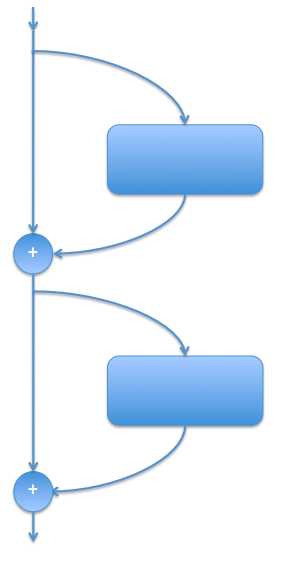
\includegraphics[width= 2.5in]{../images/resnet}
\hfill \begin{minipage}[b]{4in}
  Here we have a ``highway'' with ``diversions''.

  \bigskip
  The highway path connects input to outputs and preserves gradients.

  \bigskip
  Resnets were introduced in late 2015 (Kaiming He et al.) and revolutionized computer vision.

  \bigskip
  The resnet that won the Imagenet competition in 2015 had 152 diversions.
\end{minipage}

\slideplain{Residual Skip Connections}

$$L_{i+1} = L_i + D_i$$

\vfill
or

\vfill
$$L \;\pluseq \; D_i$$

\vfill
Here $D_i$ ``fits the residual of the identity function''

\slide{Resnet32}

\centerline{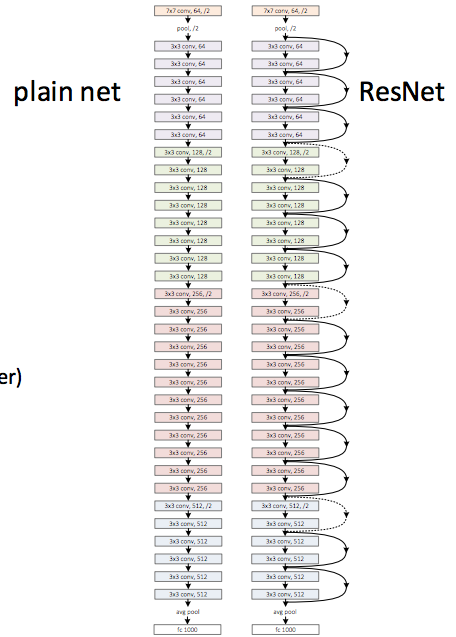
\includegraphics[height= 5.5in]{../images/ResnetStack} {\large [Kaiming He]}}

\slideplain{Deep Residual Networks}

\vfill
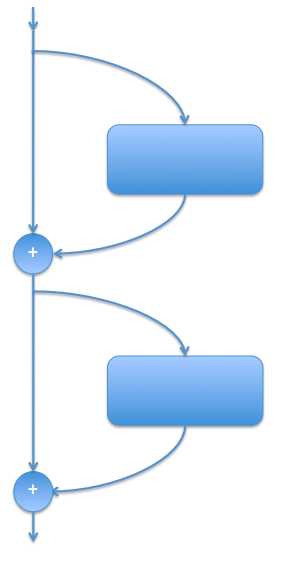
\includegraphics[width= 2.5in]{../images/resnet}
\hfill \begin{minipage}[b]{4in} As with most of deep learning, not much is known about what resnets are actually doing.
  
  \bigskip
  \bigskip
  For example, different diversions might update disjoint channels making the networks shallower than they look.

  \bigskip
  \bigskip
  They are capable of representing very general circuit topologies.
\end{minipage}

\slideplain{A Bottleneck Diversion}

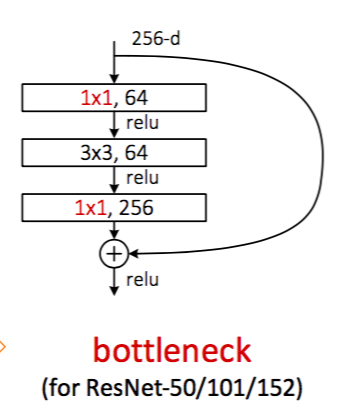
\includegraphics[width= 4.0in]{../images/bottleneck}
\hfill \begin{minipage}[b]{4in} This reduction in the number of channels used in the diversion suggests a modest update of the highway information.

  ~
  \vspace{15ex}
  ~
\end{minipage}

{\large \hspace{4em} [Kaiming He]}
\slide{Expressive Power}

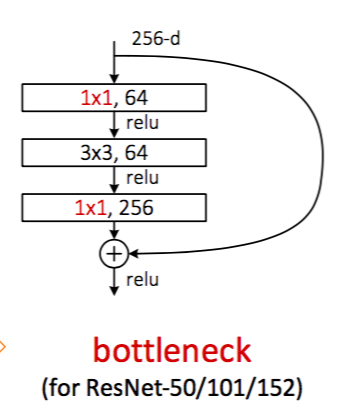
\includegraphics[width= 4.0in]{../images/bottleneck}
\hfill \begin{minipage}[b]{4in} This architecture can express fairly arbitrary state updates.

  \bigskip
  \bigskip
  Each layer has data-flow parameters.
  ~
  \vspace{8ex}
  ~
\end{minipage}

{\large \hspace{4em} [Kaiming He]}

\slideplain{Gating gives Data-Dependent Data Flow}

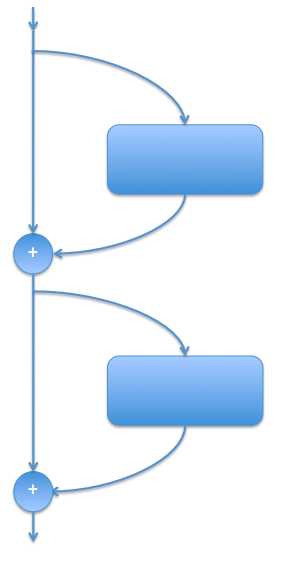
\includegraphics[width= 1.5in]{../images/resnet}
\hfill \begin{minipage}[b]{6in}
  $\begin{array}{lrcl}
    \mbox{Residual:} & y^{\ell+1} & = & y^\ell + d^\ell \\
    \\
    \mbox{LSTM:} & h^{t+1} & = & f^t \odot h^t + i^t \odot d^t \\
    \\
   \mbox{GRU:}\; &  h^{t+1} & = & f^t \odot h^t + (1-f^t)\odot d^t \\
  \end{array}$
  
  ~
  \vspace{3ex}
  ~

\end{minipage}


Resnet has data-flow parameters at each layer.

\vfill
Gated RNNs use the same parameters at each time step but use gating for data-flow control.

\slide{}
\centerline{Recurrent Neural Networks (RNNs)}

\vfill
\centerline{Speech Recognition}
\vfill
\centerline{Machine Translation}
\vfill
\centerline{Reading Comprehesion}
\vfill
\centerline{Language Modeling}

\vfill

\slide{Vanilla RNNs}

\centerline{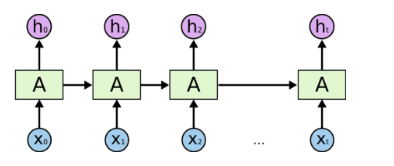
\includegraphics[width=3.5in]{../images/RNN}}
\centerline{{\large [Christopher Olah]}}

$$h[b,t+1,c_h] = \mathrm{tanh}(W[c'_h,c_h]h[b,t,c_h'] + W[c_x,c_h]x[b,t,c_x] + \beta[c_h])$$

\vfill
or
$$h^{t+1} = \mathrm{tanh}(W^{h,h}h^t + W^{x,h}x^t + \beta)$$

\vfill
or
$$h^{t+1} = \mathrm{tanh}(W^h[h^t,x^t] + \beta)$$
where $[x,y]$ denotes concatenation.

\slideplain{Exploding and Vanishing Gradients}

An RNN uses the same weights at every time step.

\vfill
If we avoid saturation of the activation functions then we get exponentially growing or shrinking eigenvectors of the weight matrix.

\vfill
Note that if the forward values are bounded by sigmoids or tanh then they cannot explode.

\vfill
However the gradients can still explode.

\slide{Exploding Gradients: Gradient Clipping}

\vfill
We can dampen the effect of exploding gradients by clipping them before applying SGD.

\vfill
$$W.\mathrm{grad} = \left\{\begin{array}{l} W.\mathrm{grad} \;\;\;\mbox{if $||W.\mathrm{grad}|| \leq n_{\mathrm{max}}$} \\
                                                      \\ \\
                                                      n_{\mathrm{max}} \; W.\mathrm{grad} / ||W.\mathrm{grad}|| \;\; \mbox{otherwise}
\end{array} \right.$$

\vfill
See {\tt torch.nn.utils.clip\_grad\_norm}

\slide{Vanishing Gradients: Highway Paths (Skip Connections)}

Modern RNNs have highway paths (skip connections).

\vfill
Unlike deep CNN layers such as Resnet, RNNs use the same parameters at each layer.

\vfill
Probably for this reason, pure residual connections are not used.

\vfill
Instead gating is used for data-dependent weighting.

\slideplain{Skip Connections}

Residual: \hspace{5em} $L_{i+1} = L_i + D_i$

\vfill
Forget Gates (LSTM): \hspace{2em} $L_{i+1} = F_i \odot L_i + I_i \odot D_i$

\vfill
Convex Gates (GRU):\hspace{1em} $L_{i+1} = F_i\odot L_i + (1-F_i) \odot D_i$

\vfill
$\odot$ is Hadamard product. This is the same as NumPy element-wise product.  However, the symbol $\odot$ is commonly used in the literature.


\anaslide{Long Short Term Memory (LSTM)}
\centerline{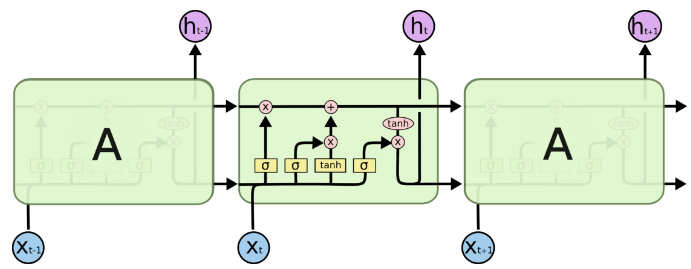
\includegraphics[width=6.0in]{../images/LSTM}}
\centerline{{\large [figure: Christopher Olah]}}

\centerline{\Large [LSTM: Hochreiter\&Shmidhuber, 1997]}

\bigskip
\bigskip
$$c^{t+1} = f^t \odot c^t + i^t \odot d^t$$

\bigskip
\bigskip
Note that if $f^t = i^t = 1$ then we have a residual connection.

\anaslideplain{Long Short Term Memory (LSTM)}

\centerline{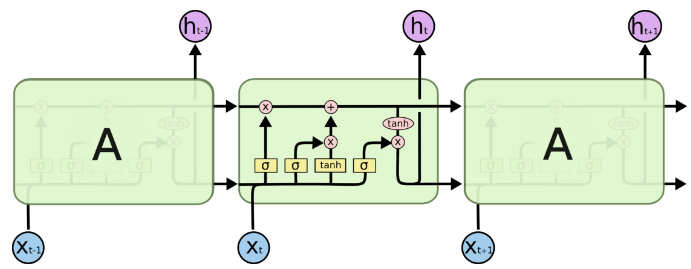
\includegraphics[width=6.0in]{../images/LSTM}}
\centerline{{\large [Christopher Olah]}}
$$c^{t+1} = f^t\odot c^t + i^t \odot d^t$$
\bigskip
$$\begin{array}{rcl}
  f^t & = & \sigma(W^f[X^t,h^t] + b^f) \\ i^t & = & \sigma(W^i[X^t,h^t]+ b^i) \\o^t & = & \sigma(W^o[X^t,h^t]+ b^0)
\end{array}
\;\;\;\;\;
\begin{array}{rcl}
d^t & = & \mathrm{tanh}(W^d[X^t,h^t] + b^d) \\ h^{t+1} & = & o^t \odot \mathrm{tanh}(c^{t+1})
\end{array}$$

\slideplain{Gated Recurrent Unity (GRU) by Cho et al. 2014}

\centerline{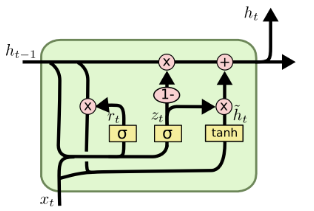
\includegraphics[width=3.0in]{../images/GRU}}
\centerline{{\huge [Christopher Olah]}}
\bigskip
$$h^{t+1} = f^t\odot h^t + (1-f^t)\odot d^t$$
\begin{eqnarray*}
  f^t & = & \sigma(W^f[x^t,h^t] + b^f) \\
  r^t & = & \sigma(W^r[x^t,h^t] + b^r)
\end{eqnarray*}
$$d^t =  \mathrm{tanh}(W^{x,d}x^t + r^t \odot (W^{h,d}h^t + b^{h,d}) + b^d)$$

\slide{GRUs vs. LSTMs}

The GRU is simpler than the LSTM.

\vfill
In TTIC31230 class projects GRUs consistently outperformed LSTMs.

\vfill
A systematic study [Collins, Dickstein and Sussulo 2016] states:

\begin{quotation}
  Our results point to the GRU as being the most learnable of gated RNNs for shallow architectures, followed by the UGRNN.
\end{quotation}


\slideplain{Update Gate RNN (UGRNN)}

$$h^{t+1} = f^t\odot h^t + (1-f^t)\odot d^t$$

$$f^t = \sigma(W^f[x^t,h^t] + b^f)$$

$$d^t =  \mathrm{tanh}(W^{d}[x^t,h^t] + b^d)$$

\slide{END}

}
\end{document}
